\chapter{Convolutional Networks Applications in Image Recognition}
% \author{Chris Rogers, Isaac Haberman, Zhengnan Huang}
% \date{February 2019}

\section{Convolution Networks for Scene Parsing and Labeling} \label{section:sceneParsing}
% Authors: Chris Rogers, Isaac Haberman
% Lecture date: 2/23/2019
Continuing the discussion of Semantic Segmentation we see how one can use convolutional neural networks to categorize and label sections of an image.  
Using this technique we're able to apply labels to many components of an image.  An example of the results can be seen in figure \ref{fig:sceneParsing} below.

\begin{figure}[!ht]
  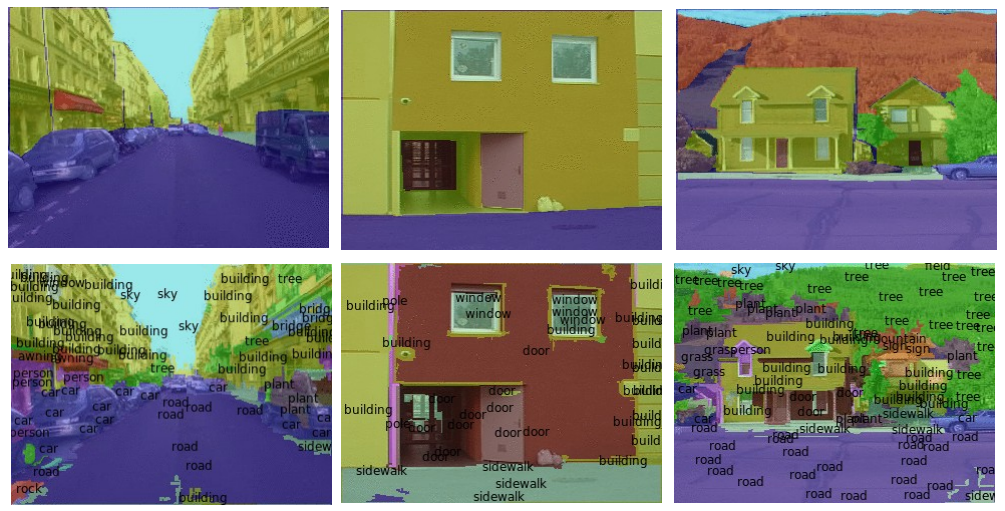
\includegraphics[width=\textwidth]{figs/SceneParsing.png}
  \caption{Example of images first segmented then labeled from class notes}
  \label{fig:sceneParsing}
\end{figure}

\subsection{Multiscale Convolution Neural Network Architecture} \label{subsection:s_multiscale}
% Authors: Chris Rogers, Isaac Haberman
% Lecture date: 2/23/2019
In the Multiscale Architecture, as described in \cite{Farabet:2013:LHF:2498740.2498895}, the model generates multiple versions of the input at different scales.  
Each version has a kernel applied to it, producing a set of features for each scale.  
The feature maps are upsampled to the largest size, and categories are predicted on the labeled images in a supervised model.  
This method allows us to pick out features in the image at a variety of scales.

In order to correctly label an image it must also be segmented.  
A \textit{superpixel} representation is created by a separate network, which over-segments the image based on local pixel information.
Each segment is assigned a category based on the "majority vote" of the features from the multiscaled network.  
An illustration of the process is shown below in figure \ref{fig:supervote}

\begin{table}[!ht]
  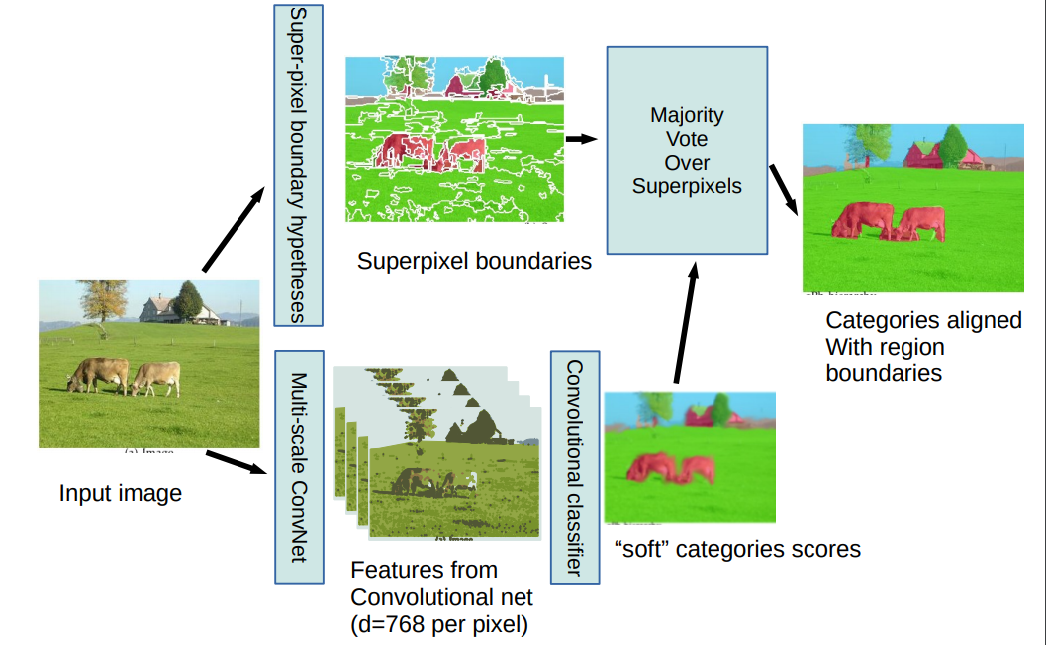
\includegraphics[width=\textwidth]{figs/SuperVote.png}
  \caption{Flow of the super-pixel/multi-scale system from class notes}
  \label{fig:supervote}
\end{table}


\subsection{RGB+Depth Images}\label{subsection:s_depth}
% Authors: Chris Rogers, Isaac Haberman
% Lecture date: 2/23/2019
In the article by \cite{DBLP:journals/corr/abs-1301-3572} we see how the approach outlined above can be applied to stills from video that captures depth information alongside the RGB image.  
The depth is treated as a a channel of another color, leaving the model otherwise as it was. 
The addition of depth is especially beneficial for static objects, like walls, whose depth stays relatively constant across the images.  


\subsection{Performance} \label{subsection:s_performance}
% Authors: Chris Rogers, Isaac Haberman
% Lecture date: 2/23/2019
A convolutional neural network can perform Scene Parsing of video at a reasonable pace.  
The network requires no post-processing and can label the images frame-by-frame.  For instance, an implementation designed by \cite{Farabet:2013:LHF:2498740.2498895} runs at 50ms/frame on Virtex-6 FPGA hardware.  
Often, the limiting factor in such implementations is network bandwidth, as much is needed to transmit the features.  
Using the Multiscale approach as described in \ref{subsection:s_multiscale}, a model produced state of the art results at a fraction of the time on the Stanford Background Dataset as seen in table \ref{fig:sbgtable}.

\begin{table}[!ht]
  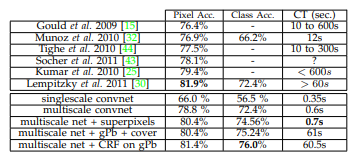
\includegraphics[width=\textwidth]{figs/StanfordBGDS8.png}
  \caption{Performance of the system on the Stanford Background dataset}
  \label{fig:sbgtable}
\end{table}

\section{Deep Convolution Networks for Object Recognition} \label{section:objectRecognition}
% Authors: Chris Rogers, Isaac Haberman
% Lecture date: 2/23/2019
Traditionally, image recognition has been done with shallow networks over hand-crafted feature-sets trained as a supervised learning problem.  
As computer power improved and GPU's became more readily available, deeper convolutional networks became more commonplace in image recognition.  
As the deeper networks were developing, large-scale labeled datasets became more readily available for model training.  
In 2012, the winning model in the ImageNet Large Scale Visual Recognition Competition, AlexNet by \cite{Krizhevsky:2012:ICD:2999134.2999257}, had a top-5 error rate of 16.4\% compared to the previous years best error rate of 25.8\%.  
With each passing year the winning model has had additional parameters and layers alongside the decreased error rate.

\subsection{Depth Inflation}\label{subsection:o_depth}
% Authors: Chris Rogers, Isaac Haberman
% Lecture date: 2/23/2019
As computational power continued to increase and new techniques for training were learned, the depth of networks continued to increase.  
With VGG from \cite{DBLP:journals/corr/SimonyanVZ13} the image is continually downsized at each layer, while the number of features is doubled, allowing it to continue to learn.  
Google (\cite{DBLP:journals/corr/SzegedyLJSRAEVR14}) produced GoogleNet, a much deeper model, with parallel layers and multiple side predictions made along the way.  
ResNet, another model used in the ImageNet competition (\cite{DBLP:journals/corr/HeZRS15}), had perhaps the largest jump in depth, and it showed that networks with over 150 layers could be successfully trained.  
ResNet was built with \textit{skip connections} or operations where a layers results were added back to previous results to prevent dying layers that normally stop the learning process.  
Since then there has been increased complexity in the models, including DenseNet by \cite{DBLP:journals/corr/HuangLW16a} which utilizes blocks of skip connections.

\subsection{Performance Comparisons}\label{subsection:o_performance}
% Authors: Chris Rogers, Isaac Haberman
% Lecture date: 2/23/2019
There are a series of techniques to evaluate networks on object recognition tasks.  
The figure below shows the Top-1 Accuracy, the computational complexity by number of operations and the model complexity by number of parameters.  
We posit that the ideal model is one in the top-left quadrant of the graph as it has both high accuracy and few operations.  
A model like ResNet-50 and Inception-v3 show some of the reasonable trade-offs needed for a good model.  
In comparison, ResNet-152 and Inception-v4 have improved accuracy over their brethren at the cost of an increased number of operations.  
DenseNet, published after the previous graph was produced, achieves a similar accuracy to ResNet-152 at a lower computational cost.  
DenseNet was further enhanced by utilizing Multiscale technique detailed in \ref{subsection:s_multiscale} alongside an early stopping condition.  Periodically, and before an image has gone through all the layers, a prediction is generated, and if the prediction probability passes a threshold the prediction is made and the operations stopped.  
The early stopping condition has been shown to operate nearly 2.6 times faster on a similar network without dynamic evaluation.

\subsection{Future work}\label{subsection:o_futureWork}
% Authors: Chris Rogers, Isaac Haberman
% Lecture date: 2/23/2019
In the race to improve performance researchers at Instagram (\cite{DBLP:journals/corr/abs-1805-00932}) have pre-trained models by attempting to predict hashtags from images on an enormous (most recently 3.5B) catalogue of images.  
As the size of their pre-training set has increased, so has their increase in accuracy.  
While the paper results are public, this pre-trained model has not been released, instead it is used as a competitive advantage for Instagram/Facebook.
 

\section{Statistics}\label{section:statistics}
%Author: Zhengnan Huang, Isaac Haberman(Editor)
%Lecture  date: 02/23/2019
Microsoft estimates the 90\% of the deep learning networks running on mobile devices are convolutional neural networks.  
Hardware and software companies are now building convolutional neural network chips that are directly integrated into smart-phones.  
In the near future, we should expect cars and children's toys to include these chips as well.

\section{Facial Recognition}\label{section:facialRecognition}
%Author: Zhengnan Huang, Isaac Haberman(Editor)
%Lecture  date: 02/23/2019
Upon initial upload of photos to Facebook, each photo is sent through several convolutional neural networks where the image is tagged and feature vectors are generated.  
The initial networks used include networks for identifying images the violate Facebook's guidelines and networks for friend and friend of friend recognition.  
This process is detailed in \cite{DBLP:journals/corr/abs-1805-00932}.

\subsubsection{Deep Face}\label{subsection:f_deepface}
%Author: Zhengnan Huang, Isaac Haberman(Editor)
%Lecture  date: 02/23/2019
Deepface is an algorithm built for face detection at Facebook and detailed in the following papers, \cite{Chopra:2005:LSM:1068507.1068961} and \cite{hadsell-chopra-lecun-06}.  
The algorithm first locates faces in an image then fits the face to a 3D model allowing the face to be unfolded and flattened.  
The unfolded face is then put through a Siamese network, where the face is then recognized.  
The siamese network is trained on a multi-part cost function where facial vectors are minimized between the same face and maximized between different faces.  
Importantly, the algorithm uses Euclidean distance, but is not squared to prevent zeroing out the gradient.  
The cost functions are defined below.


\begin{align*}
    Loss_{same face} = ||G  (x_i)  - G(x_j)|| \\
    Loss_{different faces} = Max(0, m- || G(x_i)  - G(x_j)|| \\
\end{align*}

\section{Object Detection and Localization}\label{section:objectDetection}
\subsection{Classification + Localization}\label{subsection:od_classification}
%Author: Zhengnan Huang, Isaac Haberman(Editor)
%Lecture  date: 02/23/2019
To train a convolutional neural network for object detection, we train a network on a set input scale, before implementing the network over a series of scales in a sliding window.  
The model is able to detect objects in the image and the rectangular bounding box bounding the object.  
More complex models have been used to detect the body pose of a person using these techniques.

\subsubsection{R-CNN}\label{subsection:od_rcnn}
%Author: Zhengnan Huang, Isaac Haberman(Editor)
%Lecture  date: 02/23/2019
Originally proposed in \cite{DBLP:journals/corr/GirshickDDM13}, the R-CNN uses a selective search algorithm to generate region proposals, and convolutional neural network to generate a proposed region of interest.  
A secondary classifier is then trained to classify those regions, while a regressor is trained to refine the binding box based on the region proposal location.

\begin{table}[!ht]
  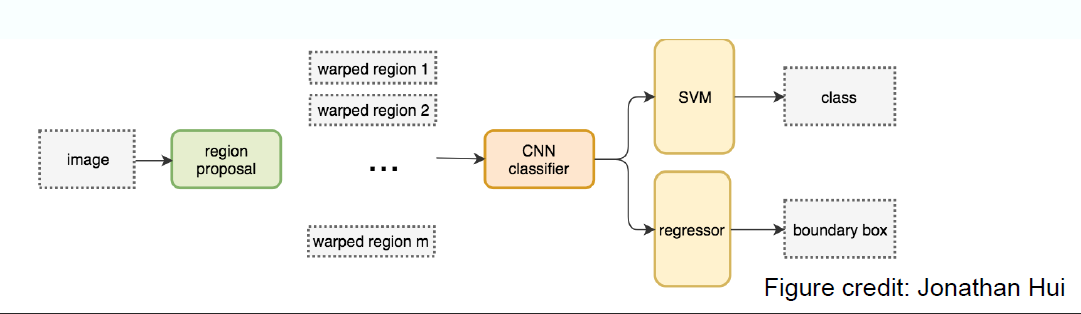
\includegraphics[width=\textwidth]{figs/r-cnn.png}
  \caption{Architecture of the R-CNN}
  \label{fig:rcnn}
\end{table}

\subsubsection{Fast R-CNN}\label{subsection:od_fastRcnn}
%Author: Zhengnan Huang, Isaac Haberman(Editor)
%Lecture  date: 02/23/2019
A more recent evolution of the R-CNN is the Fast R-CNN which feeds the image from the region of interest to the classifier.  
The regions of interest are extracted from the feature map.  

\begin{table}[!ht]
  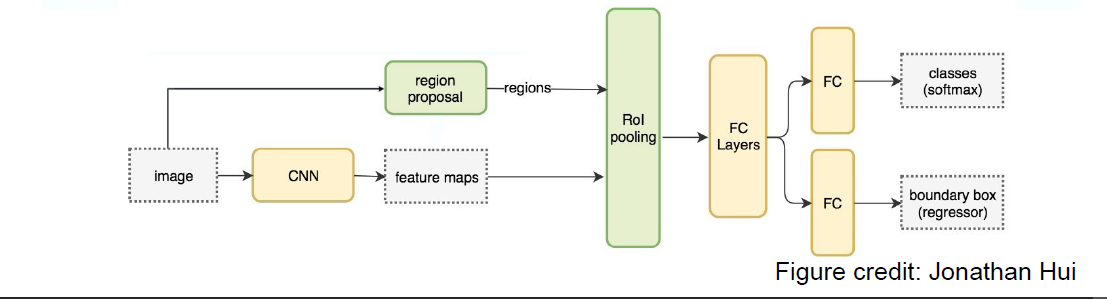
\includegraphics[width=\textwidth]{figs/fast_r-cnn.png}
  \caption{Architecture of the Fast R-CNN}
  \label{fig:fast_rcnn}
\end{table}

\subsubsection{Faster R-CNN}
%Author: Zhengnan Huang, Isaac Haberman(Editor)
%Lecture  date: 02/23/2019
More recently, the Faster R-CNN has been proposed.  
The Faster R-CNN differs from the previous Fast R-CNN as the region proposal is achieved by a neural network, instead of the selective search algorithm.

\subsubsection{YOLO}
%Author: Zhengnan Huang, Isaac Haberman(Editor)
%Lecture  date: 02/23/2019
YOLO, another convolutional neural network architecture, designed in \cite{DBLP:journals/corr/RedmonDGF15} consists of a single network that predicts the bounding boxes and perform the classification for object detection. 
The network has 24 convolutional layers and 2 fully connect layers.  
While it does not compare to the R-CNN architecture it may or may not be a faster trained algorithm.

\begin{table}[!ht]
  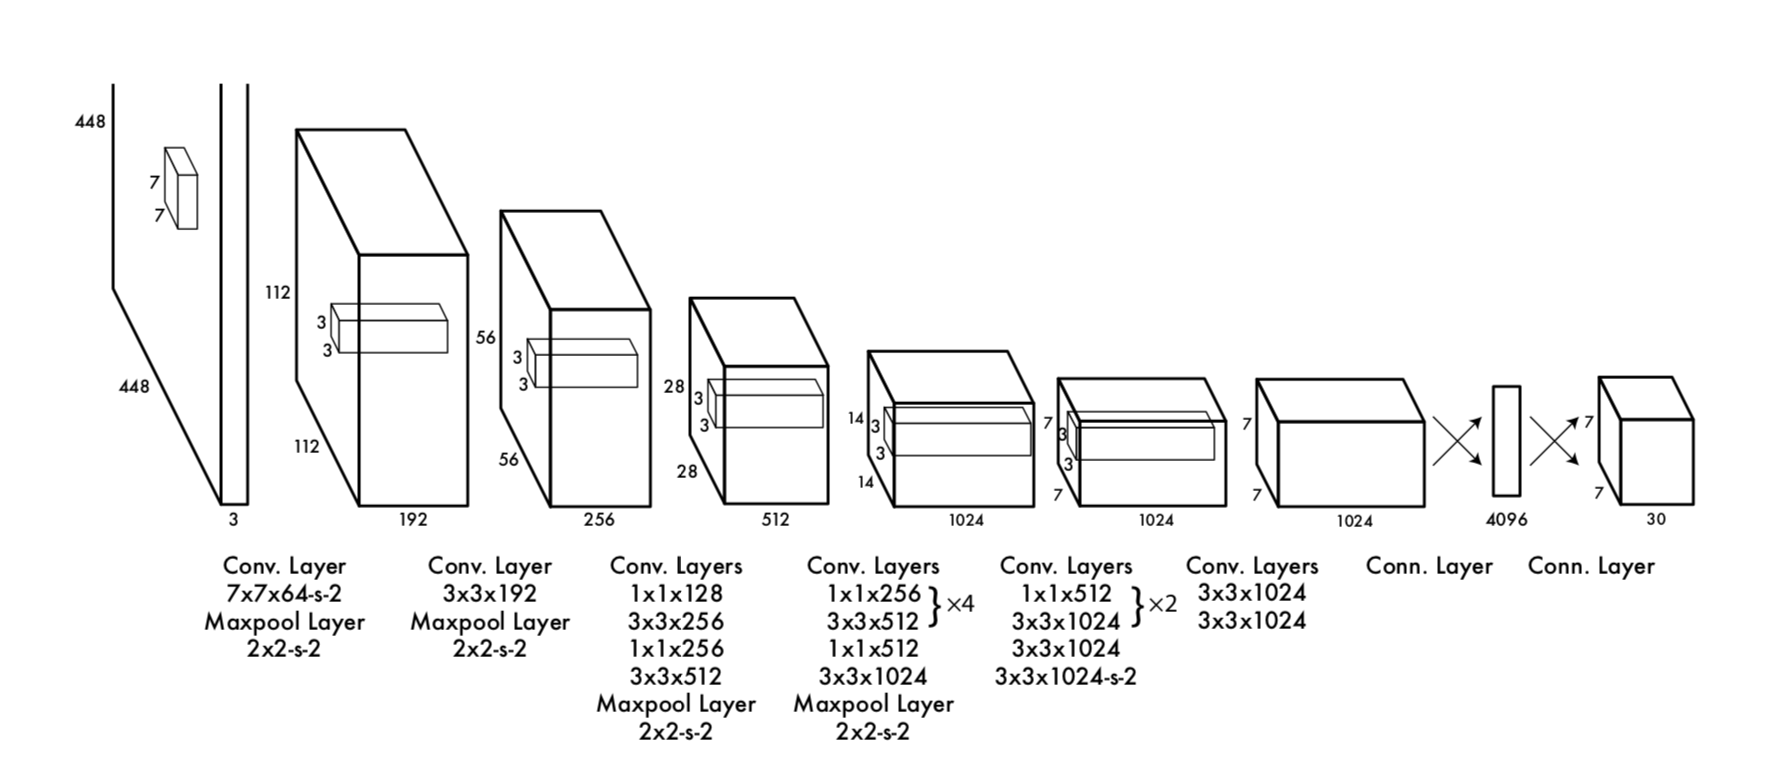
\includegraphics[width=\textwidth]{figs/yolo.png}
  \caption{Architecture of YOLO}
  \label{fig:yolo}
\end{table}


\subsubsection{DeepMask: Segmenting and Localizing Objects}
%Author: Zhengnan Huang, Isaac Haberman(Editor)
%Lecture  date: 02/23/2019
DeepMask, proposed in \cite{DBLP:journals/corr/PinheiroCD15}, is a convolutional neural network designed to produce object masks.
The region proposal is generated by a discriminative convolutional network followed by a series of convolutions and a classifier.
The classifier determines whether a pixel belongs to the object in the centre of a input image patch.

\begin{table}[!ht]
  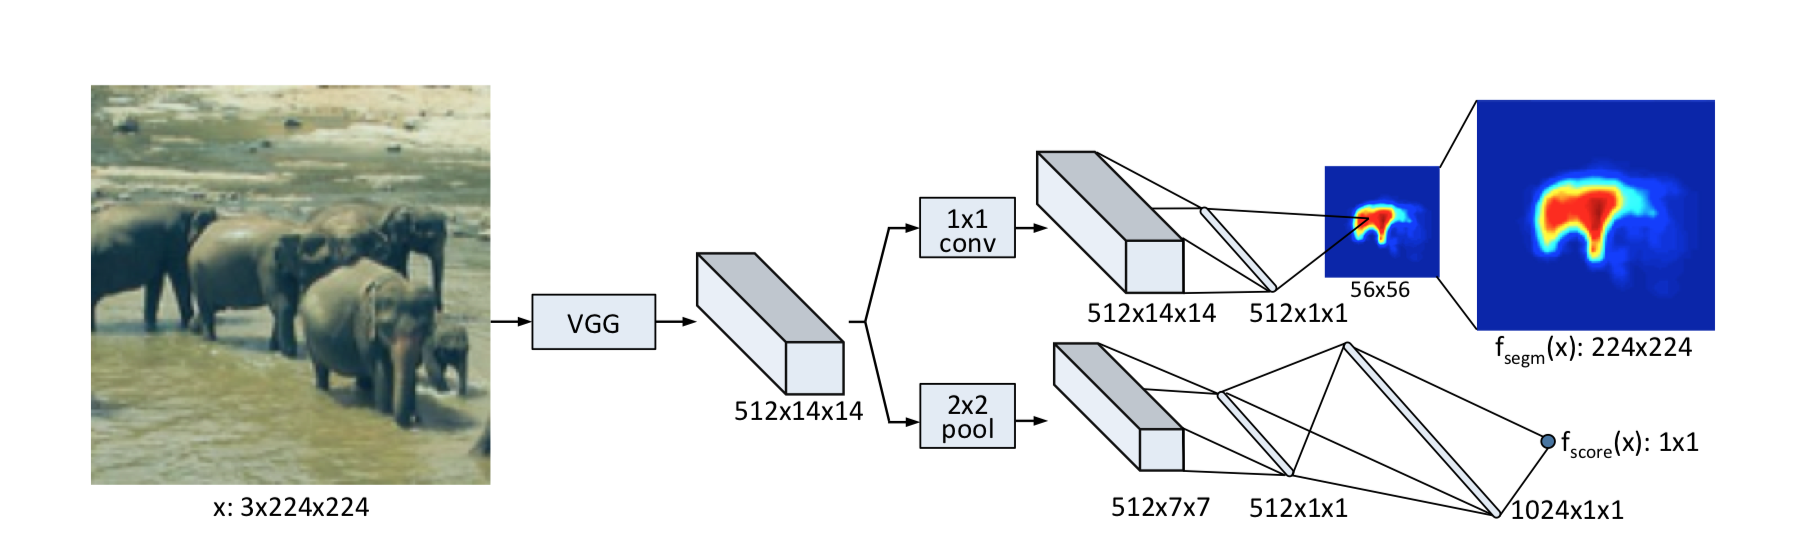
\includegraphics[width=\textwidth]{figs/deepmsk.png}
  \caption{Architecture of DeepMask}
  \label{fig:deepmsk}
\end{table}


\subsubsection{Mask R-CNN}
%Author: Zhengnan Huang, Isaac Haberman(Editor)
%Lecture  date: 02/23/2019
Mask R-CNN, \cite{DBLP:journals/corr/HeGDG17}, uses the architecture of Faster R-CNN to produce a mask for each class.
The network adds a branch to predict the object mask in parallel to the bounding box.

\begin{table}[!ht]
  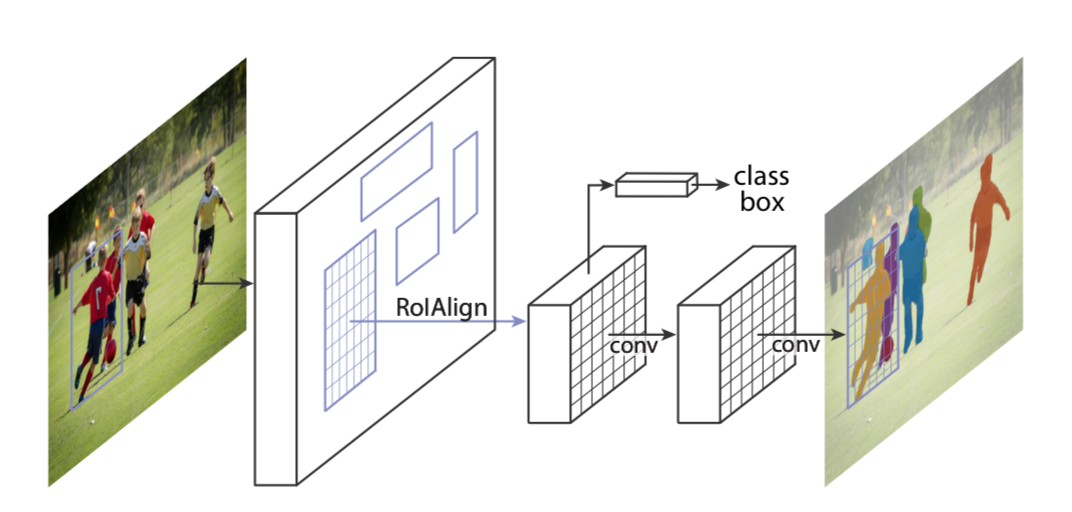
\includegraphics[width=\textwidth]{figs/maskrcnn.png}
  \caption{Architecture of Mask R-CNN}
  \label{fig:maskrcnn}
\end{table}


\subsubsection{RetinaNet}
%Author: Zhengnan Huang, Isaac Haberman(Editor)
%Lecture  date: 02/23/2019
RetinaNet, a feature pyramid network is a convolutional neural network with both down-sampling followed by upsampling with skip connections in between.
Initially proposed in \cite{DBLP:journals/corr/abs-1708-02002}, RetinaNet also uses a novel loss function.
The cross entropy loss function is utilized alongside a dynamic scaling factor that downweights the easier samples and forces the network to focus on the harder to predict examples during training.

\begin{table}[!ht]
  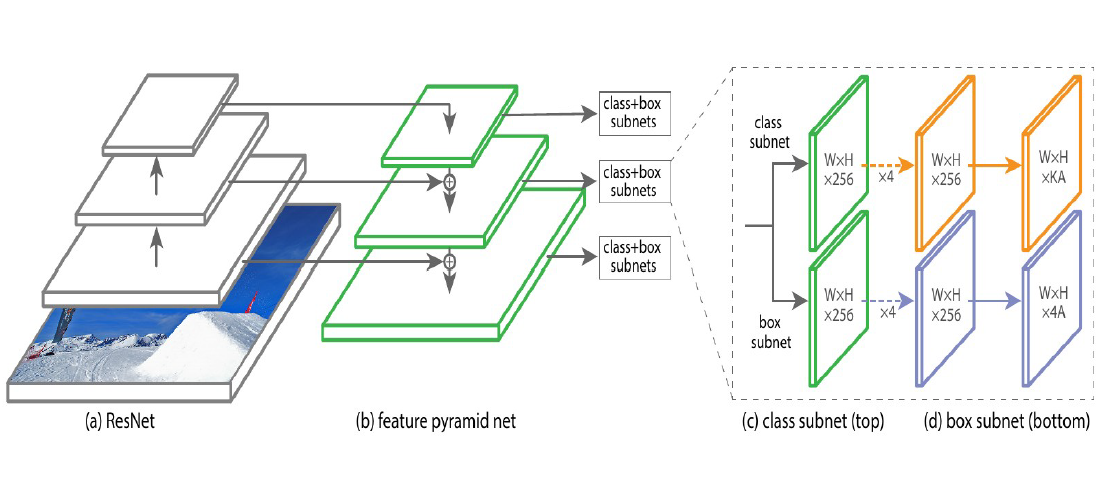
\includegraphics[width=\textwidth]{figs/retina_net.png}
  \caption{Architecture of RetinaNet}
  \label{fig:retina_net}
\end{table}


\subsubsection{DensePose: Real-Time Body Pose Estimation}
%Author: Zhengnan Huang, Isaac Haberman(Editor)
%Lecture  date: 02/23/2019
DensePose, developed by Facebook this past year in \cite{DBLP:journals/corr/abs-1809-01995}, learns the surface-based representation of the human body through a Mask R-CNN.
The system runs in real-time on a single GPU.
During network training, both fully convolutional neural networks and region-based approaches were tested, with the latter proving most effective. 

\subsection{Image Captioning}
%Author: Zhengnan Huang, Isaac Haberman(Editor)
%Lecture  date: 02/23/2019
Image Captioning was first attempted using a convolutional neural network to generate a feature vector which was used as input to an LSTM.
By training the LSTM in a supervised manner, the model can output a caption.
